\documentclass[../../main.tex]{subfiles}
\begin{document}
\begin{oframed}
  \subfile{problem}
\end{oframed}

{\bf [解答]}
\paragraph{(1)}

\begin{figure}
  % TODO: triangle ABCとその外接円@座標平面
  \caption{}
\end{figure}

$\triangle ABC$の外接円の半径1として良い．$\triangle ABC$を
\begin{align}
  A(1,0), \quad B(\cos\alpha,\sin\alpha), \quad C(\cos\beta,\sin\beta) \quad\left(0<\alpha<\beta<2\pi\right) \label{eq:1}
\end{align}
とおける．まずはこの三角形が鋭角三角形または直角三角形になる条件を考える．

\begin{figure}[htb]
  % TODO: angle A,B,Cの角度を示す図
  \caption{}
\end{figure}

上図より$\triangle ABC$のそれぞれの角は
\begin{align}
  \begin{dcases}
    \angle A = \dfrac{\pi-\alpha}{2} + \dfrac{\pi-(2\pi-\beta)}{2} = \dfrac{\beta-\alpha}{2} \\
    \angle B = \dfrac{\pi-\alpha}{2} + \dfrac{\pi-(\beta-\alpha)}{2} = \dfrac{2\pi-\beta}{2} \\
    \angle C = \dfrac{\pi-(\beta-\alpha)}{2} + \dfrac{\pi-(2\pi-\beta)}{2} = \dfrac{\alpha}{2}
  \end{dcases}
\end{align}
だから，これらが$\dfrac{\pi}{2}$より小さければ良いので
\begin{align}
  &
  \begin{dcases}
    0 < \dfrac{\beta-\alpha}{2} \le \dfrac{\pi}{2} \\
    0 < \dfrac{2\pi-\beta}{2} \le \dfrac{\pi}{2} \\
    0 < \dfrac{\alpha}{2} \le \dfrac{\pi}{2}
  \end{dcases} \\
  &
  \begin{dcases}
    \alpha < \beta \le \pi+\alpha \\
    \pi \le \beta < 2\pi \\
    0 < \alpha \le \pi
  \end{dcases} \\
  &
  \begin{dcases}
    0 < \alpha < \beta \le \pi+\alpha \\
    0 \le \alpha \le \pi
  \end{dcases} \label{eq:2}
\end{align}
である．

背理法で題意を示す．
$D$の中心を$O'$として$O'\ne O$と仮定する．$\triangle ABC$の外接円の半径が$1$でこの円は$A,B,C$を周上に含むから，$D$の半径は$1$よりも小さくなければならない．従って
\begin{align}
  |AD|\le1,\ |BD|\le1,\ |CD|\le1 \iff |AD|^2\le1,\ |BD|^2\le1,\ |CD|^2\le1 \quad(\because\text{各辺}\ge0)
\end{align}
である．$D$上の点を$(X,Y)$とおくと，これは
\begin{align}
  \begin{dcases}
    (X-1)^2+Y^2\le1 \\
    (X-\cos\alpha)^2+(Y-\sin\alpha)^2\le1 \\
    (X-\cos\beta)^2+(Y-\sin\beta)^2\le1
  \end{dcases} \label{eq:3}
\end{align}
である．そこで3円$P,Q,R$を
\begin{align}
  \begin{dcases}
    P: (X-1)^2+Y^2=1 \\
    Q: (X-\cos\alpha)^2+(Y-\sin\alpha)^2=1 \\
    R: (X-\cos\beta)^2+(Y-\sin\beta)^2=1
  \end{dcases}
\end{align}
で定める．$P,Q,R$の$(0,0)$での接線の方向ベクトルは各々$
\begin{pmatrix}0\\1
\end{pmatrix}$，$
\begin{pmatrix}-\sin\alpha\\\cos\alpha
\end{pmatrix}$，$
\begin{pmatrix}\sin\beta\\-\cos\beta
\end{pmatrix}$だから，これを図示すると下図のようになる．

\begin{figure}[htb]
  % TODO: 円P,Q,Rと(0,0)での接線ベクトル
  \caption{}
\end{figure}

$P$は$Q$の左側，$Q$は$R$の上側，$R$は$P$の左側にあるから，$P,Q,R$の共有点は$O(0,0)$のみ，つまり
\begin{align}
  \text{\cref{eq:3}} \iff (X,Y)=(0,0)
\end{align}
であるが，これは$O'\ne O$に反し矛盾する．以上から題意は示された．\qed

\subparagraph{(2)}

(1)のベクトル図から，$\triangle ABC$が鈍角三角形になれば\cref{eq:3}の領域が$(0,0)$以外に広がり，$D\ne O$となる．したがって，
\begin{align}
  \triangle ABC\text{が非鈍角三角形}\iff D=O \label{eq:4}
\end{align}
となる．したがって，$\triangle ABC$が鈍角三角形になるような$C$の軌跡を求めれば良い．対称性から，$0\le x,\ 0<y$で考える．また$C(x,y)$とする．

\subparagraph{$1^\circ$ $1<x$の時}

$\angle CAB>\pi/2$となり，$\triangle ABC$は鈍角三角形である．

\subparagraph{$2^\circ$ $0\le x\le1$の時}

$\angle CAB\le\pi/2,\ \angle CBA\le\pi/2$だから，$\angle ACB>\pi/2$となる条件をしらべれば良い．このような条件は
\begin{align}
  x^2+y^2<1
\end{align}
である．
\casesend

以上$1^\circ,2^\circ$から，$0\le x,\ 0<y$では，題意の条件は $1<x$ or $x^2+y^2<1$だから，対称性から求める領域式は
\begin{align}
  |x|>1 \ \text{または}\ x^2+y^2<1 \quad(y\ne0)
\end{align}
であり，制約$x^2+y^2\le4$とあわせて図示して下図斜線部（境界は$x^2+y^2=4$のみ含み，$x$軸は含まず）．

\begin{figure}[htb]
  \begin{center}
    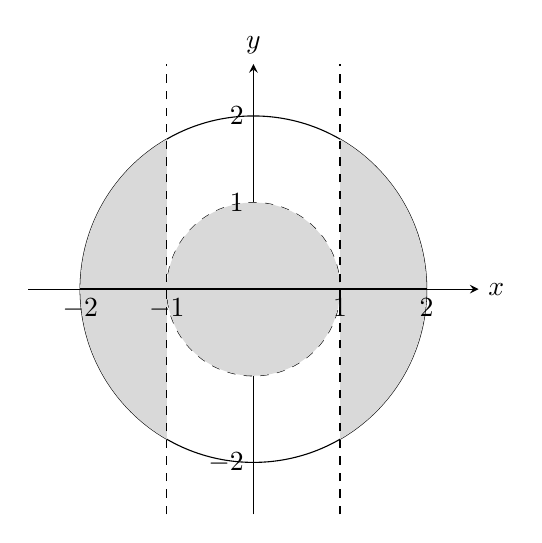
\begin{tikzpicture}[scale=1.1, >=stealth]
      % 座標軸
      \draw[->] (-2.6,0) -- (2.6,0) node[right] {$x$};
      \draw[->] (0,-2.6) -- (0,2.6) node[above] {$y$};
      % 制約 x^2+y^2<=4 (境界含む) と 補助円 x^2+y^2=1 (境界含まず)
      \draw (0,0) circle (2);
      \draw[dashed] (0,0) circle (1);
      % 領域: |x|>1 または x^2+y^2<1 (かつ x^2+y^2<=4)
      \begin{scope}
        \clip (0,0) circle (2);
        \fill[gray!30] (-2.6,-2.6) rectangle (-1,2.6);
        \fill[gray!30] (1,-2.6) rectangle (2.6,2.6);
        \fill[gray!30] (0,0) circle (1);
      \end{scope}
      \draw[dashed] (-1,-2.6) -- (-1,2.6);
      \draw[dashed] (1,-2.6) -- (1,2.6);
      \draw[thick] (-2,0) -- (2,0);
      \node[below] at (-2,0) {$-2$};
      \node[below] at (-1,0) {$-1$};
      \node[below] at (1,0) {$1$};
      \node[below] at (2,0) {$2$};
      \node[left] at (0,2) {$2$};
      \node[left] at (0,1) {$1$};
      \node[left] at (0,-2) {$-2$};
    \end{tikzpicture}
  \end{center}
  \caption{条件を満たす領域の図示（斜線部）}
\end{figure}

\newpage

\end{document}
